% ============================================================
\begin{frame}{Source Mode (200 compounds): Structures sorted by IC$_{50}$ (1--10)}
  \centering
  \tiny
  \begin{tabular}{r c l l c c c}
    \toprule
    \textbf{Rank} & \textbf{Structure} & \textbf{Source mode} & \textbf{Family} & \textbf{IC$_{50}$ ($\mu$M)} & \textbf{pIC$_{50}$} & \textbf{cLogP} \\
    \midrule
    1 & 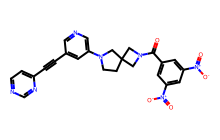
\includegraphics[width=0.9cm]{figures/gate1_structures/rank_001.png} & plain & reinvent\_pubchem & 0.78 & 6.11 & 2.44 \\
    2 & 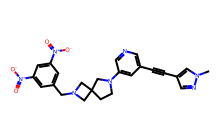
\includegraphics[width=0.9cm]{figures/gate1_structures/rank_002.png} & plain & reinvent\_pubchem & 0.78 & 6.11 & 2.74 \\
    3 & 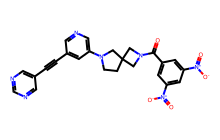
\includegraphics[width=0.9cm]{figures/gate1_structures/rank_003.png} & plain & reinvent\_pubchem & 0.78 & 6.11 & 2.44 \\
    4 & 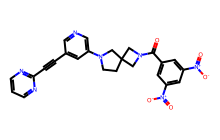
\includegraphics[width=0.9cm]{figures/gate1_structures/rank_004.png} & plain & reinvent\_pubchem & 0.85 & 6.07 & 2.44 \\
    5 & 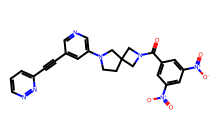
\includegraphics[width=0.9cm]{figures/gate1_structures/rank_005.png} & plain & reinvent\_pubchem & 0.85 & 6.07 & 2.44 \\
    6 & 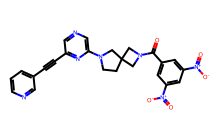
\includegraphics[width=0.9cm]{figures/gate1_structures/rank_006.png} & plain & reinvent\_pubchem & 0.85 & 6.07 & 2.44 \\
    7 & 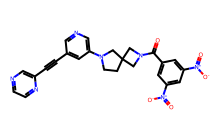
\includegraphics[width=0.9cm]{figures/gate1_structures/rank_007.png} & plain & reinvent\_pubchem & 0.85 & 6.07 & 2.44 \\
    8 & 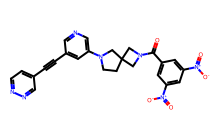
\includegraphics[width=0.9cm]{figures/gate1_structures/rank_008.png} & plain & reinvent\_pubchem & 0.85 & 6.07 & 2.44 \\
    9 & 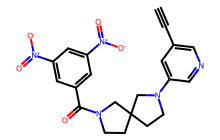
\includegraphics[width=0.9cm]{figures/gate1_structures/rank_009.png} & plain & reinvent\_pubchem & 0.85 & 6.07 & 2.62 \\
    10 & 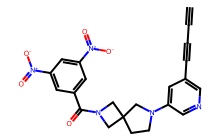
\includegraphics[width=0.9cm]{figures/gate1_structures/rank_010.png} & plain & reinvent\_pubchem & 0.85 & 6.07 & 2.24 \\
    \bottomrule
  \end{tabular}
\end{frame}

% ============================================================
\begin{frame}{Source Mode (200 compounds): Structures sorted by IC$_{50}$ (11--20)}
  \centering
  \tiny
  \begin{tabular}{r c l l c c c}
    \toprule
    \textbf{Rank} & \textbf{Structure} & \textbf{Source mode} & \textbf{Family} & \textbf{IC$_{50}$ ($\mu$M)} & \textbf{pIC$_{50}$} & \textbf{cLogP} \\
    \midrule
    11 & 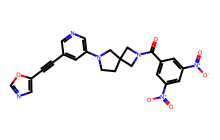
\includegraphics[width=0.9cm]{figures/gate1_structures/rank_011.png} & plain & reinvent\_pubchem & 0.85 & 6.07 & 2.64 \\
    12 & 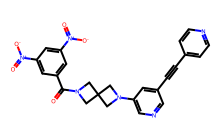
\includegraphics[width=0.9cm]{figures/gate1_structures/rank_012.png} & plain & reinvent\_pubchem & 0.85 & 6.07 & 2.66 \\
    13 & 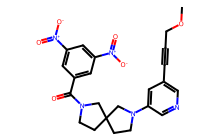
\includegraphics[width=0.9cm]{figures/gate1_structures/rank_013.png} & plain & reinvent\_pubchem & 0.85 & 6.07 & 2.64 \\
    14 & 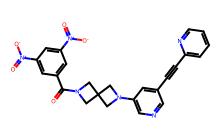
\includegraphics[width=0.9cm]{figures/gate1_structures/rank_014.png} & plain & reinvent\_pubchem & 0.85 & 6.07 & 2.66 \\
    15 & 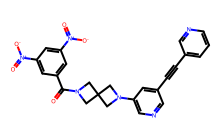
\includegraphics[width=0.9cm]{figures/gate1_structures/rank_015.png} & plain & reinvent\_pubchem & 0.85 & 6.07 & 2.66 \\
    16 & 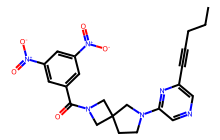
\includegraphics[width=0.9cm]{figures/gate1_structures/rank_016.png} & plain & reinvent\_pubchem & 0.85 & 6.07 & 2.80 \\
    17 & 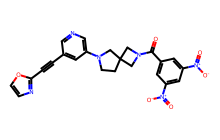
\includegraphics[width=0.9cm]{figures/gate1_structures/rank_017.png} & plain & reinvent\_pubchem & 0.85 & 6.07 & 2.64 \\
    18 & 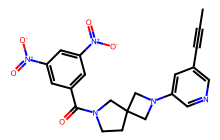
\includegraphics[width=0.9cm]{figures/gate1_structures/rank_018.png} & plain & reinvent\_pubchem & 0.85 & 6.07 & 2.62 \\
    19 & 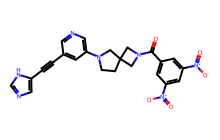
\includegraphics[width=0.9cm]{figures/gate1_structures/rank_019.png} & plain & reinvent\_pubchem & 0.85 & 6.07 & 2.37 \\
    20 & 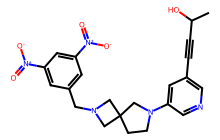
\includegraphics[width=0.9cm]{figures/gate1_structures/rank_020.png} & plain & reinvent\_pubchem & 0.85 & 6.07 & 2.34 \\
    \bottomrule
  \end{tabular}
\end{frame}

% ============================================================
\begin{frame}{Source Mode (200 compounds): Structures sorted by IC$_{50}$ (21--30)}
  \centering
  \tiny
  \begin{tabular}{r c l l c c c}
    \toprule
    \textbf{Rank} & \textbf{Structure} & \textbf{Source mode} & \textbf{Family} & \textbf{IC$_{50}$ ($\mu$M)} & \textbf{pIC$_{50}$} & \textbf{cLogP} \\
    \midrule
    21 & 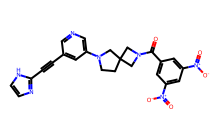
\includegraphics[width=0.9cm]{figures/gate1_structures/rank_021.png} & plain & reinvent\_pubchem & 0.85 & 6.07 & 2.37 \\
    22 & 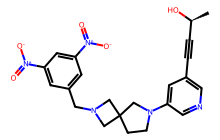
\includegraphics[width=0.9cm]{figures/gate1_structures/rank_022.png} & plain & reinvent\_pubchem & 0.85 & 6.07 & 2.34 \\
    23 & 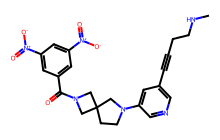
\includegraphics[width=0.9cm]{figures/gate1_structures/rank_023.png} & plain & reinvent\_pubchem & 0.85 & 6.07 & 2.21 \\
    24 & 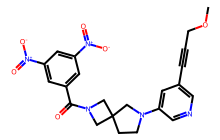
\includegraphics[width=0.9cm]{figures/gate1_structures/rank_024.png} & plain & reinvent\_pubchem & 0.85 & 6.07 & 2.25 \\
    25 & 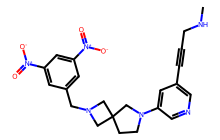
\includegraphics[width=0.9cm]{figures/gate1_structures/rank_025.png} & plain & reinvent\_pubchem & 0.85 & 6.07 & 2.18 \\
    26 & 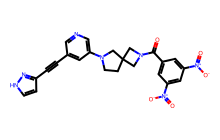
\includegraphics[width=0.9cm]{figures/gate1_structures/rank_026.png} & plain & reinvent\_pubchem & 0.85 & 6.07 & 2.37 \\
    27 & 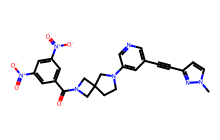
\includegraphics[width=0.9cm]{figures/gate1_structures/rank_027.png} & plain & reinvent\_pubchem & 0.85 & 6.07 & 2.38 \\
    28 & 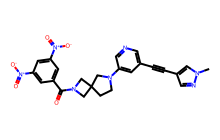
\includegraphics[width=0.9cm]{figures/gate1_structures/rank_028.png} & plain & reinvent\_pubchem & 0.85 & 6.07 & 2.38 \\
    29 & 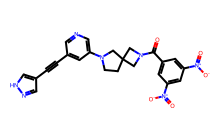
\includegraphics[width=0.9cm]{figures/gate1_structures/rank_029.png} & plain & reinvent\_pubchem & 0.85 & 6.07 & 2.37 \\
    30 & 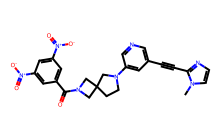
\includegraphics[width=0.9cm]{figures/gate1_structures/rank_030.png} & plain & reinvent\_pubchem & 0.85 & 6.07 & 2.38 \\
    \bottomrule
  \end{tabular}
\end{frame}

% ============================================================
\begin{frame}{Source Mode (200 compounds): Structures sorted by IC$_{50}$ (31--40)}
  \centering
  \tiny
  \begin{tabular}{r c l l c c c}
    \toprule
    \textbf{Rank} & \textbf{Structure} & \textbf{Source mode} & \textbf{Family} & \textbf{IC$_{50}$ ($\mu$M)} & \textbf{pIC$_{50}$} & \textbf{cLogP} \\
    \midrule
    31 & 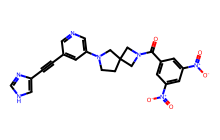
\includegraphics[width=0.9cm]{figures/gate1_structures/rank_031.png} & plain & reinvent\_pubchem & 0.85 & 6.07 & 2.37 \\
    32 & 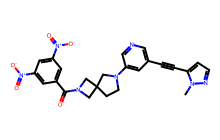
\includegraphics[width=0.9cm]{figures/gate1_structures/rank_032.png} & plain & reinvent\_pubchem & 0.85 & 6.07 & 2.38 \\
    33 & 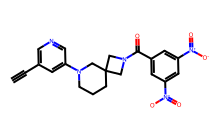
\includegraphics[width=0.9cm]{figures/gate1_structures/rank_033.png} & plain & reinvent\_pubchem & 0.95 & 6.02 & 2.62 \\
    34 & 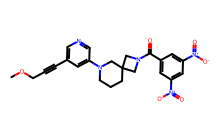
\includegraphics[width=0.9cm]{figures/gate1_structures/rank_034.png} & plain & reinvent\_pubchem & 0.95 & 6.02 & 2.64 \\
    35 & 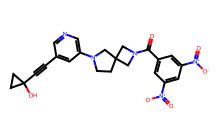
\includegraphics[width=0.9cm]{figures/gate1_structures/rank_035.png} & plain & reinvent\_pubchem & 1.04 & 5.98 & 2.13 \\
    36 & 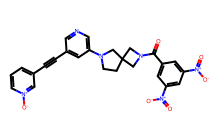
\includegraphics[width=0.9cm]{figures/gate1_structures/rank_036.png} & plain & reinvent\_pubchem & 1.13 & 5.95 & 2.28 \\
    37 & 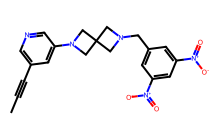
\includegraphics[width=0.9cm]{figures/gate1_structures/rank_037.png} & plain & reinvent\_pubchem & 1.24 & 5.91 & 2.59 \\
    38 & 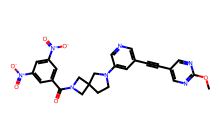
\includegraphics[width=0.9cm]{figures/gate1_structures/rank_038.png} & plain & reinvent\_pubchem & 1.27 & 5.89 & 2.45 \\
    39 & 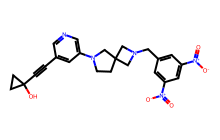
\includegraphics[width=0.9cm]{figures/gate1_structures/rank_039.png} & plain & reinvent\_pubchem & 1.31 & 5.88 & 2.49 \\
    40 & 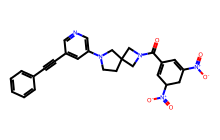
\includegraphics[width=0.9cm]{figures/gate1_structures/rank_040.png} & plain & reinvent\_pubchem & 1.31 & 5.88 & 2.66 \\
    \bottomrule
  \end{tabular}
\end{frame}

% ============================================================
\begin{frame}{Source Mode (200 compounds): Structures sorted by IC$_{50}$ (41--50)}
  \centering
  \tiny
  \begin{tabular}{r c l l c c c}
    \toprule
    \textbf{Rank} & \textbf{Structure} & \textbf{Source mode} & \textbf{Family} & \textbf{IC$_{50}$ ($\mu$M)} & \textbf{pIC$_{50}$} & \textbf{cLogP} \\
    \midrule
    41 & 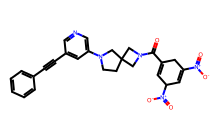
\includegraphics[width=0.9cm]{figures/gate1_structures/rank_041.png} & plain & reinvent\_pubchem & 1.31 & 5.88 & 2.66 \\
    42 & 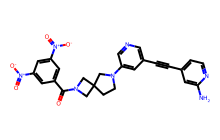
\includegraphics[width=0.9cm]{figures/gate1_structures/rank_042.png} & plain & reinvent\_pubchem & 1.50 & 5.83 & 2.63 \\
    43 & 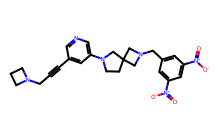
\includegraphics[width=0.9cm]{figures/gate1_structures/rank_043.png} & plain & reinvent\_pubchem & 1.54 & 5.81 & 2.67 \\
    44 & 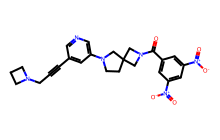
\includegraphics[width=0.9cm]{figures/gate1_structures/rank_044.png} & plain & reinvent\_pubchem & 1.54 & 5.81 & 2.31 \\
    45 & 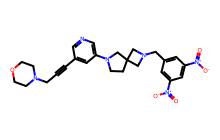
\includegraphics[width=0.9cm]{figures/gate1_structures/rank_045.png} & plain & reinvent\_pubchem & 1.54 & 5.81 & 2.29 \\
    46 & 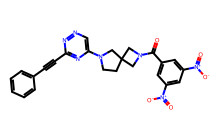
\includegraphics[width=0.9cm]{figures/gate1_structures/rank_046.png} & plain & reinvent\_pubchem & 1.94 & 5.71 & 2.44 \\
    47 & 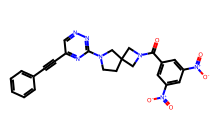
\includegraphics[width=0.9cm]{figures/gate1_structures/rank_047.png} & plain & reinvent\_pubchem & 1.94 & 5.71 & 2.44 \\
    48 & 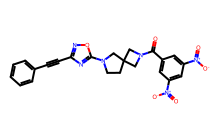
\includegraphics[width=0.9cm]{figures/gate1_structures/rank_048.png} & plain & reinvent\_pubchem & 1.94 & 5.71 & 2.64 \\
    49 & 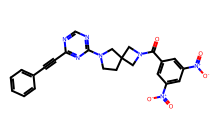
\includegraphics[width=0.9cm]{figures/gate1_structures/rank_049.png} & plain & reinvent\_pubchem & 1.94 & 5.71 & 2.44 \\
    50 & 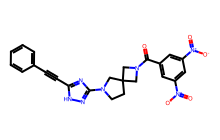
\includegraphics[width=0.9cm]{figures/gate1_structures/rank_050.png} & plain & reinvent\_pubchem & 1.94 & 5.71 & 2.37 \\
    \bottomrule
  \end{tabular}
\end{frame}

% ============================================================
\begin{frame}{Source Mode (200 compounds): Structures sorted by IC$_{50}$ (51--60)}
  \centering
  \tiny
  \begin{tabular}{r c l l c c c}
    \toprule
    \textbf{Rank} & \textbf{Structure} & \textbf{Source mode} & \textbf{Family} & \textbf{IC$_{50}$ ($\mu$M)} & \textbf{pIC$_{50}$} & \textbf{cLogP} \\
    \midrule
    51 & 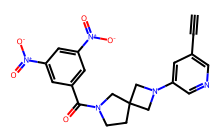
\includegraphics[width=0.9cm]{figures/gate1_structures/rank_051.png} & plain & reinvent\_pubchem & 1.94 & 5.71 & 2.23 \\
    52 & 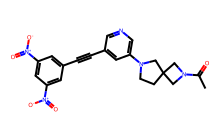
\includegraphics[width=0.9cm]{figures/gate1_structures/rank_052.png} & plain & reinvent\_pubchem & 1.94 & 5.71 & 2.36 \\
    53 & 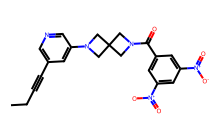
\includegraphics[width=0.9cm]{figures/gate1_structures/rank_053.png} & plain & reinvent\_pubchem & 1.94 & 5.71 & 2.62 \\
    54 & 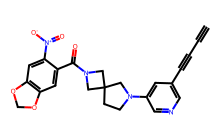
\includegraphics[width=0.9cm]{figures/gate1_structures/rank_054.png} & plain & reinvent\_pubchem & 2.49 & 5.60 & 2.06 \\
    55 & 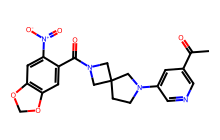
\includegraphics[width=0.9cm]{figures/gate1_structures/rank_055.png} & plain & reinvent\_pubchem & 2.49 & 5.60 & 2.27 \\
    56 & 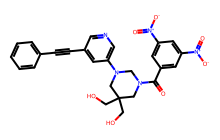
\includegraphics[width=0.9cm]{figures/gate1_structures/rank_056.png} & plain & reinvent\_pubchem & 2.71 & 5.57 & 2.19 \\
    57 & 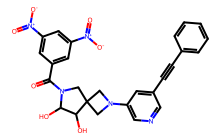
\includegraphics[width=0.9cm]{figures/gate1_structures/rank_057.png} & plain & reinvent\_pubchem & 2.73 & 5.56 & 1.94 \\
    58 & 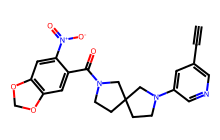
\includegraphics[width=0.9cm]{figures/gate1_structures/rank_058.png} & plain & reinvent\_pubchem & 2.77 & 5.56 & 2.44 \\
    59 & 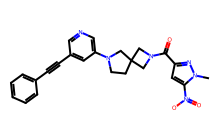
\includegraphics[width=0.9cm]{figures/gate1_structures/rank_059.png} & plain & reinvent\_pubchem & 2.88 & 5.54 & 2.48 \\
    60 & 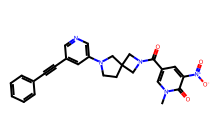
\includegraphics[width=0.9cm]{figures/gate1_structures/rank_060.png} & plain & reinvent\_pubchem & 2.88 & 5.54 & 2.44 \\
    \bottomrule
  \end{tabular}
\end{frame}

% ============================================================
\begin{frame}{Source Mode (200 compounds): Structures sorted by IC$_{50}$ (61--70)}
  \centering
  \tiny
  \begin{tabular}{r c l l c c c}
    \toprule
    \textbf{Rank} & \textbf{Structure} & \textbf{Source mode} & \textbf{Family} & \textbf{IC$_{50}$ ($\mu$M)} & \textbf{pIC$_{50}$} & \textbf{cLogP} \\
    \midrule
    61 & 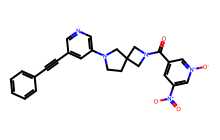
\includegraphics[width=0.9cm]{figures/gate1_structures/rank_061.png} & plain & reinvent\_pubchem & 2.88 & 5.54 & 2.38 \\
    62 & 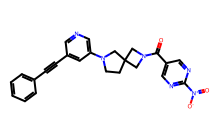
\includegraphics[width=0.9cm]{figures/gate1_structures/rank_062.png} & plain & reinvent\_pubchem & 2.88 & 5.54 & 2.53 \\
    63 & 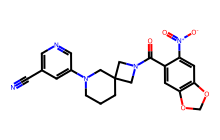
\includegraphics[width=0.9cm]{figures/gate1_structures/rank_063.png} & plain & reinvent\_pubchem & 2.91 & 5.54 & 2.33 \\
    64 & 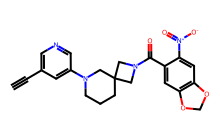
\includegraphics[width=0.9cm]{figures/gate1_structures/rank_064.png} & plain & reinvent\_pubchem & 2.91 & 5.54 & 2.44 \\
    65 & 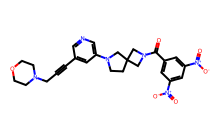
\includegraphics[width=0.9cm]{figures/gate1_structures/rank_065.png} & plain & reinvent\_pubchem & 3.14 & 5.50 & 1.93 \\
    66 & 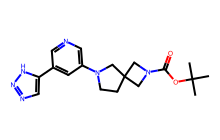
\includegraphics[width=0.9cm]{figures/gate1_structures/rank_066.png} & plain & reinvent\_pubchem & 3.53 & 5.45 & 2.31 \\
    67 & 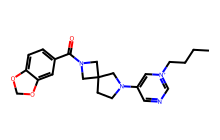
\includegraphics[width=0.9cm]{figures/gate1_structures/rank_067.png} & mol2mol\_scaffold & nitro\_bioisostere\_campaign & 3.61 & 5.44 & 2.25 \\
    68 & 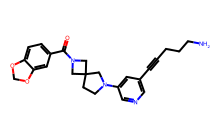
\includegraphics[width=0.9cm]{figures/gate1_structures/rank_068.png} & plain & reinvent\_pubchem & 3.61 & 5.44 & 2.25 \\
    69 & 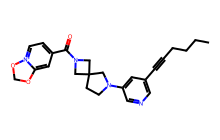
\includegraphics[width=0.9cm]{figures/gate1_structures/rank_069.png} & mol2mol\_scaffold & nitro\_bioisostere\_campaign & 3.61 & 5.44 & 2.04 \\
    70 & 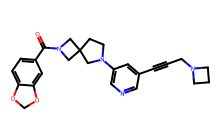
\includegraphics[width=0.9cm]{figures/gate1_structures/rank_070.png} & plain & reinvent\_pubchem & 3.61 & 5.44 & 2.22 \\
    \bottomrule
  \end{tabular}
\end{frame}

% ============================================================
\begin{frame}{Source Mode (200 compounds): Structures sorted by IC$_{50}$ (71--80)}
  \centering
  \tiny
  \begin{tabular}{r c l l c c c}
    \toprule
    \textbf{Rank} & \textbf{Structure} & \textbf{Source mode} & \textbf{Family} & \textbf{IC$_{50}$ ($\mu$M)} & \textbf{pIC$_{50}$} & \textbf{cLogP} \\
    \midrule
    71 & 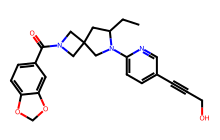
\includegraphics[width=0.9cm]{figures/gate1_structures/rank_071.png} & mol2mol\_scaffold\_generic & nitro\_bioisostere\_campaign & 3.61 & 5.44 & 2.29 \\
    72 & 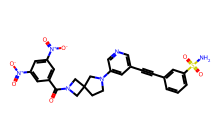
\includegraphics[width=0.9cm]{figures/gate1_structures/rank_072.png} & plain & reinvent\_pubchem & 3.76 & 5.42 & 2.30 \\
    73 & 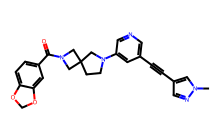
\includegraphics[width=0.9cm]{figures/gate1_structures/rank_073.png} & plain & reinvent\_pubchem & 3.80 & 5.42 & 2.30 \\
    74 & 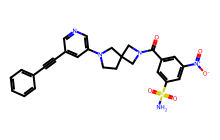
\includegraphics[width=0.9cm]{figures/gate1_structures/rank_074.png} & plain & reinvent\_pubchem & 3.84 & 5.42 & 2.39 \\
    75 & 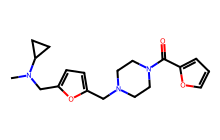
\includegraphics[width=0.9cm]{figures/gate1_structures/rank_075.png} & plain & reinvent & 3.96 & 5.40 & 2.42 \\
    76 & 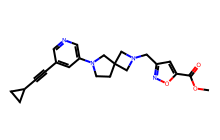
\includegraphics[width=0.9cm]{figures/gate1_structures/rank_076.png} & mol2mol\_similarity & nitro\_bioisostere\_campaign & 4.03 & 5.39 & 2.33 \\
    77 & 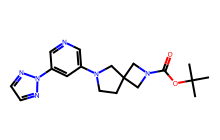
\includegraphics[width=0.9cm]{figures/gate1_structures/rank_077.png} & plain & reinvent\_pubchem & 4.03 & 5.39 & 2.11 \\
    78 & 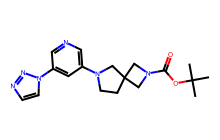
\includegraphics[width=0.9cm]{figures/gate1_structures/rank_078.png} & plain & reinvent\_pubchem & 4.03 & 5.39 & 2.11 \\
    79 & 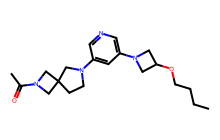
\includegraphics[width=0.9cm]{figures/gate1_structures/rank_079.png} & plain & reinvent\_pubchem & 4.03 & 5.39 & 2.15 \\
    80 & 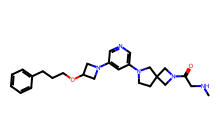
\includegraphics[width=0.9cm]{figures/gate1_structures/rank_080.png} & plain & reinvent\_pubchem & 4.03 & 5.39 & 2.18 \\
    \bottomrule
  \end{tabular}
\end{frame}

% ============================================================
\begin{frame}{Source Mode (200 compounds): Structures sorted by IC$_{50}$ (81--90)}
  \centering
  \tiny
  \begin{tabular}{r c l l c c c}
    \toprule
    \textbf{Rank} & \textbf{Structure} & \textbf{Source mode} & \textbf{Family} & \textbf{IC$_{50}$ ($\mu$M)} & \textbf{pIC$_{50}$} & \textbf{cLogP} \\
    \midrule
    81 & 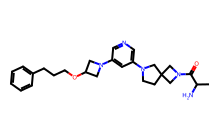
\includegraphics[width=0.9cm]{figures/gate1_structures/rank_081.png} & plain & reinvent\_pubchem & 4.03 & 5.39 & 2.31 \\
    82 & 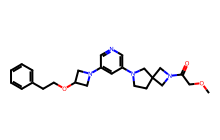
\includegraphics[width=0.9cm]{figures/gate1_structures/rank_082.png} & plain & reinvent\_pubchem & 4.03 & 5.39 & 2.21 \\
    83 & 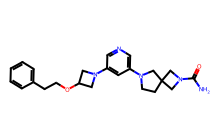
\includegraphics[width=0.9cm]{figures/gate1_structures/rank_083.png} & plain & reinvent\_pubchem & 4.03 & 5.39 & 2.12 \\
    84 & 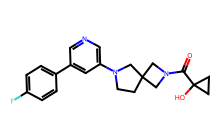
\includegraphics[width=0.9cm]{figures/gate1_structures/rank_084.png} & plain & reinvent\_pubchem & 4.03 & 5.39 & 2.45 \\
    85 & 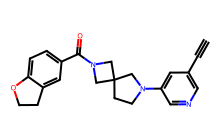
\includegraphics[width=0.9cm]{figures/gate1_structures/rank_085.png} & mol2mol\_scaffold\_generic & nitro\_bioisostere\_campaign & 4.03 & 5.39 & 2.35 \\
    86 & 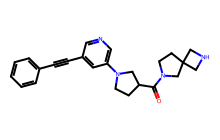
\includegraphics[width=0.9cm]{figures/gate1_structures/rank_086.png} & plain & reinvent\_pubchem & 4.03 & 5.39 & 2.13 \\
    87 & 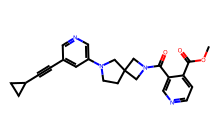
\includegraphics[width=0.9cm]{figures/gate1_structures/rank_087.png} & mol2mol\_similarity & nitro\_bioisostere\_campaign & 4.03 & 5.39 & 2.38 \\
    88 & 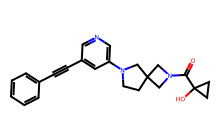
\includegraphics[width=0.9cm]{figures/gate1_structures/rank_088.png} & plain & reinvent\_pubchem & 4.03 & 5.39 & 2.04 \\
    89 & 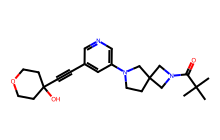
\includegraphics[width=0.9cm]{figures/gate1_structures/rank_089.png} & mol2mol\_similarity & nitro\_bioisostere\_campaign & 4.03 & 5.39 & 2.06 \\
    90 & 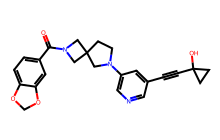
\includegraphics[width=0.9cm]{figures/gate1_structures/rank_090.png} & plain & reinvent\_pubchem & 4.18 & 5.38 & 2.04 \\
    \bottomrule
  \end{tabular}
\end{frame}

% ============================================================
\begin{frame}{Source Mode (200 compounds): Structures sorted by IC$_{50}$ (91--100)}
  \centering
  \tiny
  \begin{tabular}{r c l l c c c}
    \toprule
    \textbf{Rank} & \textbf{Structure} & \textbf{Source mode} & \textbf{Family} & \textbf{IC$_{50}$ ($\mu$M)} & \textbf{pIC$_{50}$} & \textbf{cLogP} \\
    \midrule
    91 & 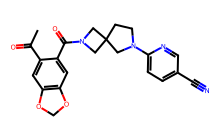
\includegraphics[width=0.9cm]{figures/gate1_structures/rank_091.png} & mol2mol\_scaffold\_generic & nitro\_bioisostere\_campaign & 4.18 & 5.38 & 2.24 \\
    92 & 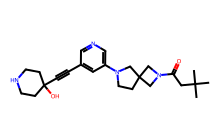
\includegraphics[width=0.9cm]{figures/gate1_structures/rank_092.png} & mol2mol\_similarity & nitro\_bioisostere\_campaign & 4.23 & 5.37 & 2.02 \\
    93 & 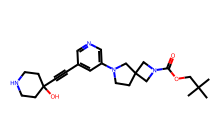
\includegraphics[width=0.9cm]{figures/gate1_structures/rank_093.png} & mol2mol\_similarity & nitro\_bioisostere\_campaign & 4.23 & 5.37 & 2.24 \\
    94 & 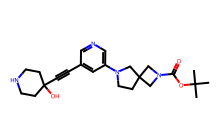
\includegraphics[width=0.9cm]{figures/gate1_structures/rank_094.png} & mol2mol\_similarity & nitro\_bioisostere\_campaign & 4.23 & 5.37 & 1.99 \\
    95 & 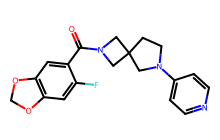
\includegraphics[width=0.9cm]{figures/gate1_structures/rank_095.png} & mol2mol\_scaffold & nitro\_bioisostere\_campaign & 4.24 & 5.37 & 2.30 \\
    96 & 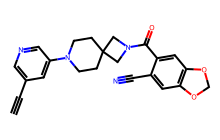
\includegraphics[width=0.9cm]{figures/gate1_structures/rank_096.png} & mol2mol\_similarity & nitro\_bioisostere\_campaign & 4.24 & 5.37 & 2.41 \\
    97 & 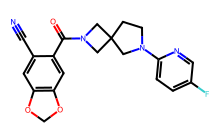
\includegraphics[width=0.9cm]{figures/gate1_structures/rank_097.png} & mol2mol\_scaffold\_generic & nitro\_bioisostere\_campaign & 4.24 & 5.37 & 2.17 \\
    98 & 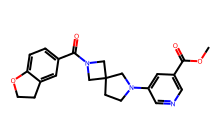
\includegraphics[width=0.9cm]{figures/gate1_structures/rank_098.png} & mol2mol\_scaffold\_generic & nitro\_bioisostere\_campaign & 4.24 & 5.37 & 2.16 \\
    99 & 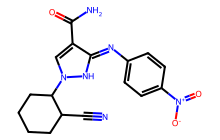
\includegraphics[width=0.9cm]{figures/gate1_structures/rank_099.png} & curriculum\_learning & reinvent & 4.33 & 5.36 & 2.31 \\
    100 & 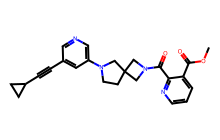
\includegraphics[width=0.9cm]{figures/gate1_structures/rank_100.png} & mol2mol\_similarity & nitro\_bioisostere\_campaign & 4.41 & 5.36 & 2.38 \\
    \bottomrule
  \end{tabular}
\end{frame}

% ============================================================
\begin{frame}{Source Mode (200 compounds): Structures sorted by IC$_{50}$ (101--110)}
  \centering
  \tiny
  \begin{tabular}{r c l l c c c}
    \toprule
    \textbf{Rank} & \textbf{Structure} & \textbf{Source mode} & \textbf{Family} & \textbf{IC$_{50}$ ($\mu$M)} & \textbf{pIC$_{50}$} & \textbf{cLogP} \\
    \midrule
    101 & 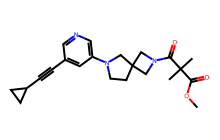
\includegraphics[width=0.9cm]{figures/gate1_structures/rank_101.png} & mol2mol\_similarity & nitro\_bioisostere\_campaign & 4.41 & 5.36 & 2.08 \\
    102 & 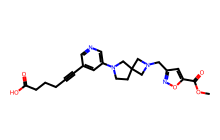
\includegraphics[width=0.9cm]{figures/gate1_structures/rank_102.png} & mol2mol\_similarity & nitro\_bioisostere\_campaign & 4.41 & 5.36 & 2.17 \\
    103 & 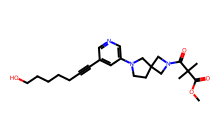
\includegraphics[width=0.9cm]{figures/gate1_structures/rank_103.png} & mol2mol\_similarity & nitro\_bioisostere\_campaign & 4.41 & 5.36 & 2.22 \\
    104 & 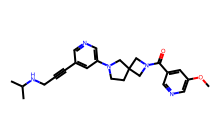
\includegraphics[width=0.9cm]{figures/gate1_structures/rank_104.png} & mol2mol\_scaffold\_generic & nitro\_bioisostere\_campaign & 4.41 & 5.36 & 2.19 \\
    105 & 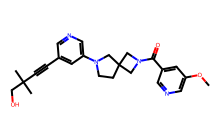
\includegraphics[width=0.9cm]{figures/gate1_structures/rank_105.png} & mol2mol\_scaffold\_generic & nitro\_bioisostere\_campaign & 4.41 & 5.36 & 2.21 \\
    106 & 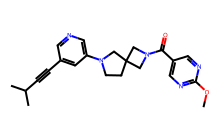
\includegraphics[width=0.9cm]{figures/gate1_structures/rank_106.png} & mol2mol\_scaffold\_generic & nitro\_bioisostere\_campaign & 4.41 & 5.36 & 2.24 \\
    107 & 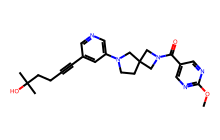
\includegraphics[width=0.9cm]{figures/gate1_structures/rank_107.png} & mol2mol\_scaffold\_generic & nitro\_bioisostere\_campaign & 4.41 & 5.36 & 2.14 \\
    108 & 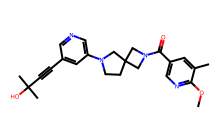
\includegraphics[width=0.9cm]{figures/gate1_structures/rank_108.png} & mol2mol\_scaffold\_generic & nitro\_bioisostere\_campaign & 4.41 & 5.36 & 2.27 \\
    109 & 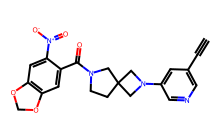
\includegraphics[width=0.9cm]{figures/gate1_structures/rank_109.png} & plain & reinvent\_pubchem & 4.44 & 5.35 & 2.05 \\
    110 & 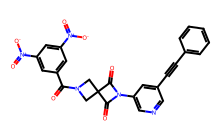
\includegraphics[width=0.9cm]{figures/gate1_structures/rank_110.png} & plain & reinvent\_pubchem & 4.55 & 5.34 & 2.31 \\
    \bottomrule
  \end{tabular}
\end{frame}

% ============================================================
\begin{frame}{Source Mode (200 compounds): Structures sorted by IC$_{50}$ (111--120)}
  \centering
  \tiny
  \begin{tabular}{r c l l c c c}
    \toprule
    \textbf{Rank} & \textbf{Structure} & \textbf{Source mode} & \textbf{Family} & \textbf{IC$_{50}$ ($\mu$M)} & \textbf{pIC$_{50}$} & \textbf{cLogP} \\
    \midrule
    111 & 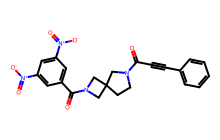
\includegraphics[width=0.9cm]{figures/gate1_structures/rank_111.png} & plain & reinvent\_pubchem & 4.55 & 5.34 & 2.23 \\
    112 & 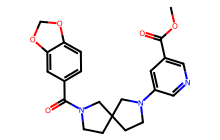
\includegraphics[width=0.9cm]{figures/gate1_structures/rank_112.png} & mol2mol\_similarity & nitro\_bioisostere\_campaign & 4.58 & 5.34 & 2.34 \\
    113 & 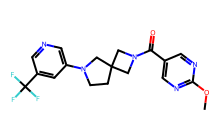
\includegraphics[width=0.9cm]{figures/gate1_structures/rank_113.png} & mol2mol\_scaffold\_generic & nitro\_bioisostere\_campaign & 4.64 & 5.33 & 2.25 \\
    114 & 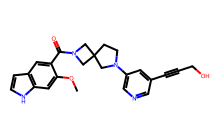
\includegraphics[width=0.9cm]{figures/gate1_structures/rank_114.png} & mol2mol\_similarity & nitro\_bioisostere\_campaign & 4.70 & 5.33 & 2.27 \\
    115 & 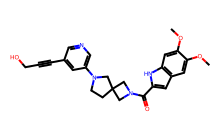
\includegraphics[width=0.9cm]{figures/gate1_structures/rank_115.png} & mol2mol\_similarity & nitro\_bioisostere\_campaign & 4.71 & 5.33 & 2.28 \\
    116 & 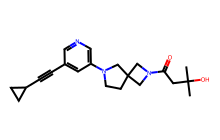
\includegraphics[width=0.9cm]{figures/gate1_structures/rank_116.png} & mol2mol\_similarity & nitro\_bioisostere\_campaign & 4.72 & 5.33 & 2.04 \\
    117 & 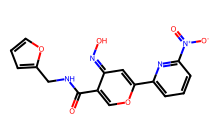
\includegraphics[width=0.9cm]{figures/gate1_structures/rank_117.png} & curriculum\_learning & reinvent & 4.77 & 5.32 & 2.06 \\
    118 & 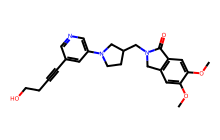
\includegraphics[width=0.9cm]{figures/gate1_structures/rank_118.png} & mol2mol\_similarity & nitro\_bioisostere\_campaign & 4.77 & 5.32 & 2.32 \\
    119 & 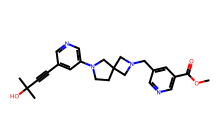
\includegraphics[width=0.9cm]{figures/gate1_structures/rank_119.png} & mol2mol\_scaffold\_generic & nitro\_bioisostere\_campaign & 4.98 & 5.30 & 2.10 \\
    120 & 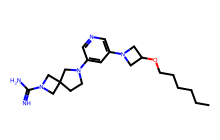
\includegraphics[width=0.9cm]{figures/gate1_structures/rank_120.png} & plain & reinvent\_pubchem & 4.98 & 5.30 & 2.27 \\
    \bottomrule
  \end{tabular}
\end{frame}

% ============================================================
\begin{frame}{Source Mode (200 compounds): Structures sorted by IC$_{50}$ (121--130)}
  \centering
  \tiny
  \begin{tabular}{r c l l c c c}
    \toprule
    \textbf{Rank} & \textbf{Structure} & \textbf{Source mode} & \textbf{Family} & \textbf{IC$_{50}$ ($\mu$M)} & \textbf{pIC$_{50}$} & \textbf{cLogP} \\
    \midrule
    121 & 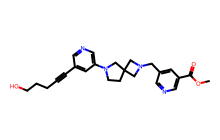
\includegraphics[width=0.9cm]{figures/gate1_structures/rank_121.png} & mol2mol\_scaffold\_generic & nitro\_bioisostere\_campaign & 4.98 & 5.30 & 2.10 \\
    122 & 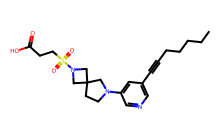
\includegraphics[width=0.9cm]{figures/gate1_structures/rank_122.png} & mol2mol\_similarity & nitro\_bioisostere\_campaign & 4.98 & 5.30 & 2.33 \\
    123 & 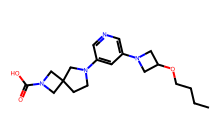
\includegraphics[width=0.9cm]{figures/gate1_structures/rank_123.png} & plain & reinvent\_pubchem & 5.14 & 5.29 & 2.28 \\
    124 & 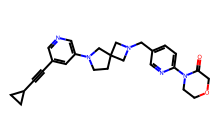
\includegraphics[width=0.9cm]{figures/gate1_structures/rank_124.png} & mol2mol\_similarity & nitro\_bioisostere\_campaign & 5.14 & 5.29 & 2.31 \\
    125 & 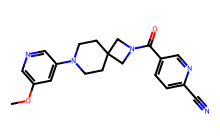
\includegraphics[width=0.9cm]{figures/gate1_structures/rank_125.png} & mol2mol\_similarity & nitro\_bioisostere\_campaign & 5.18 & 5.29 & 2.10 \\
    126 & 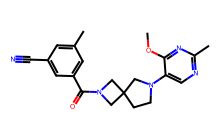
\includegraphics[width=0.9cm]{figures/gate1_structures/rank_126.png} & mol2mol\_scaffold\_generic & nitro\_bioisostere\_campaign & 5.18 & 5.29 & 2.33 \\
    127 & 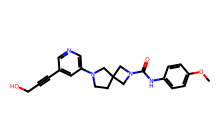
\includegraphics[width=0.9cm]{figures/gate1_structures/rank_127.png} & mol2mol\_similarity & nitro\_bioisostere\_campaign & 5.18 & 5.29 & 2.18 \\
    128 & 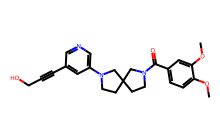
\includegraphics[width=0.9cm]{figures/gate1_structures/rank_128.png} & mol2mol\_similarity & nitro\_bioisostere\_campaign & 5.25 & 5.28 & 2.19 \\
    129 & 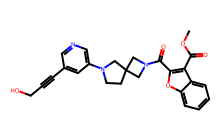
\includegraphics[width=0.9cm]{figures/gate1_structures/rank_129.png} & mol2mol\_similarity & nitro\_bioisostere\_campaign & 5.28 & 5.28 & 2.31 \\
    130 & 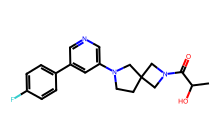
\includegraphics[width=0.9cm]{figures/gate1_structures/rank_130.png} & plain & reinvent\_pubchem & 5.31 & 5.28 & 2.31 \\
    \bottomrule
  \end{tabular}
\end{frame}

% ============================================================
\begin{frame}{Source Mode (200 compounds): Structures sorted by IC$_{50}$ (131--140)}
  \centering
  \tiny
  \begin{tabular}{r c l l c c c}
    \toprule
    \textbf{Rank} & \textbf{Structure} & \textbf{Source mode} & \textbf{Family} & \textbf{IC$_{50}$ ($\mu$M)} & \textbf{pIC$_{50}$} & \textbf{cLogP} \\
    \midrule
    131 & 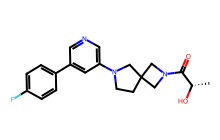
\includegraphics[width=0.9cm]{figures/gate1_structures/rank_131.png} & plain & reinvent\_pubchem & 5.53 & 5.26 & 2.31 \\
    132 & 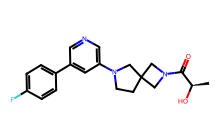
\includegraphics[width=0.9cm]{figures/gate1_structures/rank_132.png} & plain & reinvent\_pubchem & 5.53 & 5.26 & 2.31 \\
    133 & 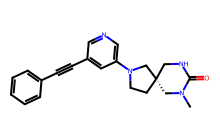
\includegraphics[width=0.9cm]{figures/gate1_structures/rank_133.png} & plain & reinvent\_pubchem & 5.53 & 5.26 & 2.33 \\
    134 & 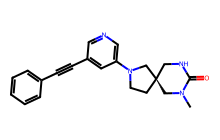
\includegraphics[width=0.9cm]{figures/gate1_structures/rank_134.png} & plain & reinvent\_pubchem & 5.53 & 5.26 & 2.33 \\
    135 & 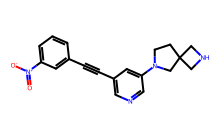
\includegraphics[width=0.9cm]{figures/gate1_structures/rank_135.png} & plain & reinvent\_pubchem & 5.53 & 5.26 & 2.19 \\
    136 & 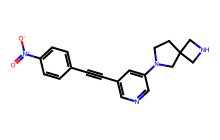
\includegraphics[width=0.9cm]{figures/gate1_structures/rank_136.png} & plain & reinvent\_pubchem & 5.53 & 5.26 & 2.19 \\
    137 & 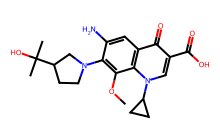
\includegraphics[width=0.9cm]{figures/gate1_structures/rank_137.png} & plain & reinvent & 5.55 & 5.26 & 2.22 \\
    138 & 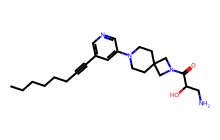
\includegraphics[width=0.9cm]{figures/gate1_structures/rank_138.png} & mol2mol\_similarity & nitro\_bioisostere\_campaign & 5.57 & 5.25 & 2.15 \\
    139 & 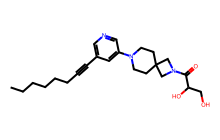
\includegraphics[width=0.9cm]{figures/gate1_structures/rank_139.png} & mol2mol\_similarity & nitro\_bioisostere\_campaign & 5.57 & 5.25 & 2.19 \\
    140 & 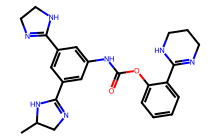
\includegraphics[width=0.9cm]{figures/gate1_structures/rank_140.png} & curriculum\_learning & reinvent & 5.76 & 5.24 & 2.13 \\
    \bottomrule
  \end{tabular}
\end{frame}

% ============================================================
\begin{frame}{Source Mode (200 compounds): Structures sorted by IC$_{50}$ (141--150)}
  \centering
  \tiny
  \begin{tabular}{r c l l c c c}
    \toprule
    \textbf{Rank} & \textbf{Structure} & \textbf{Source mode} & \textbf{Family} & \textbf{IC$_{50}$ ($\mu$M)} & \textbf{pIC$_{50}$} & \textbf{cLogP} \\
    \midrule
    141 & 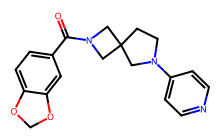
\includegraphics[width=0.9cm]{figures/gate1_structures/rank_141.png} & mol2mol\_scaffold\_generic & nitro\_bioisostere\_campaign & 5.83 & 5.23 & 2.16 \\
    142 & 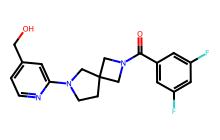
\includegraphics[width=0.9cm]{figures/gate1_structures/rank_142.png} & mol2mol\_scaffold\_generic & nitro\_bioisostere\_campaign & 6.03 & 5.22 & 2.20 \\
    143 & 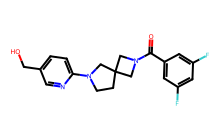
\includegraphics[width=0.9cm]{figures/gate1_structures/rank_143.png} & mol2mol\_scaffold\_generic & nitro\_bioisostere\_campaign & 6.03 & 5.22 & 2.20 \\
    144 & 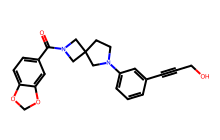
\includegraphics[width=0.9cm]{figures/gate1_structures/rank_144.png} & mol2mol\_scaffold\_generic & nitro\_bioisostere\_campaign & 6.09 & 5.22 & 2.11 \\
    145 & 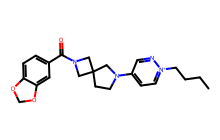
\includegraphics[width=0.9cm]{figures/gate1_structures/rank_145.png} & mol2mol\_scaffold\_generic & nitro\_bioisostere\_campaign & 6.09 & 5.22 & 2.25 \\
    146 & 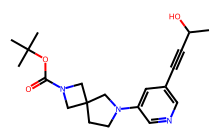
\includegraphics[width=0.9cm]{figures/gate1_structures/rank_146.png} & plain & reinvent\_pubchem & 6.21 & 5.21 & 2.26 \\
    147 & 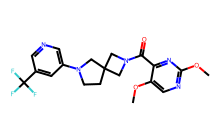
\includegraphics[width=0.9cm]{figures/gate1_structures/rank_147.png} & mol2mol\_scaffold\_generic & nitro\_bioisostere\_campaign & 6.28 & 5.20 & 2.26 \\
    148 & 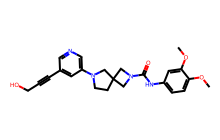
\includegraphics[width=0.9cm]{figures/gate1_structures/rank_148.png} & mol2mol\_similarity & nitro\_bioisostere\_campaign & 6.28 & 5.20 & 2.19 \\
    149 & 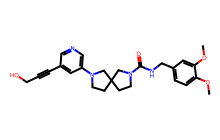
\includegraphics[width=0.9cm]{figures/gate1_structures/rank_149.png} & mol2mol\_similarity & nitro\_bioisostere\_campaign & 6.28 & 5.20 & 2.25 \\
    150 & 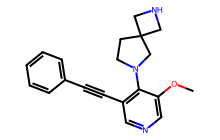
\includegraphics[width=0.9cm]{figures/gate1_structures/rank_150.png} & plain & reinvent\_pubchem & 6.35 & 5.20 & 2.29 \\
    \bottomrule
  \end{tabular}
\end{frame}

% ============================================================
\begin{frame}{Source Mode (200 compounds): Structures sorted by IC$_{50}$ (151--160)}
  \centering
  \tiny
  \begin{tabular}{r c l l c c c}
    \toprule
    \textbf{Rank} & \textbf{Structure} & \textbf{Source mode} & \textbf{Family} & \textbf{IC$_{50}$ ($\mu$M)} & \textbf{pIC$_{50}$} & \textbf{cLogP} \\
    \midrule
    151 & 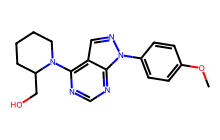
\includegraphics[width=0.9cm]{figures/gate1_structures/rank_151.png} & plain & reinvent & 6.35 & 5.20 & 2.18 \\
    152 & 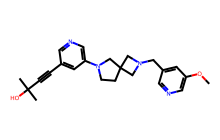
\includegraphics[width=0.9cm]{figures/gate1_structures/rank_152.png} & mol2mol\_scaffold\_generic & nitro\_bioisostere\_campaign & 6.64 & 5.18 & 2.32 \\
    153 & 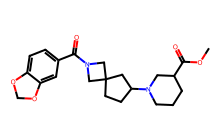
\includegraphics[width=0.9cm]{figures/gate1_structures/rank_153.png} & mol2mol\_scaffold\_generic & nitro\_bioisostere\_campaign & 6.68 & 5.18 & 2.29 \\
    154 & 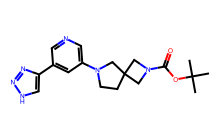
\includegraphics[width=0.9cm]{figures/gate1_structures/rank_154.png} & plain & reinvent\_pubchem & 7.38 & 5.13 & 2.31 \\
    155 & 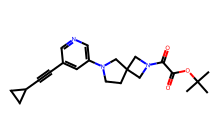
\includegraphics[width=0.9cm]{figures/gate1_structures/rank_155.png} & mol2mol\_similarity & nitro\_bioisostere\_campaign & 7.38 & 5.13 & 2.22 \\
    156 & 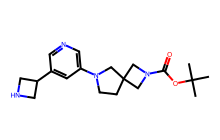
\includegraphics[width=0.9cm]{figures/gate1_structures/rank_156.png} & plain & reinvent\_pubchem & 7.38 & 5.13 & 2.22 \\
    157 & 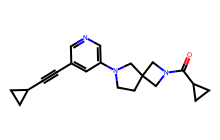
\includegraphics[width=0.9cm]{figures/gate1_structures/rank_157.png} & mol2mol\_similarity & nitro\_bioisostere\_campaign & 7.45 & 5.13 & 2.29 \\
    158 & 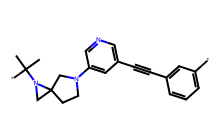
\includegraphics[width=0.9cm]{figures/gate1_structures/rank_158.png} & curriculum\_learning & linkinvent\_transformer\_pubchem & 7.52 & 5.12 & 2.21 \\
    159 & 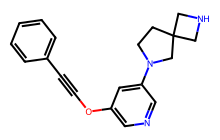
\includegraphics[width=0.9cm]{figures/gate1_structures/rank_159.png} & plain & reinvent\_pubchem & 7.61 & 5.12 & 2.27 \\
    160 & 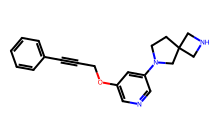
\includegraphics[width=0.9cm]{figures/gate1_structures/rank_160.png} & plain & reinvent\_pubchem & 7.61 & 5.12 & 2.31 \\
    \bottomrule
  \end{tabular}
\end{frame}

% ============================================================
\begin{frame}{Source Mode (200 compounds): Structures sorted by IC$_{50}$ (161--170)}
  \centering
  \tiny
  \begin{tabular}{r c l l c c c}
    \toprule
    \textbf{Rank} & \textbf{Structure} & \textbf{Source mode} & \textbf{Family} & \textbf{IC$_{50}$ ($\mu$M)} & \textbf{pIC$_{50}$} & \textbf{cLogP} \\
    \midrule
    161 & 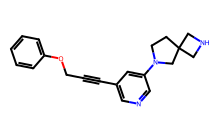
\includegraphics[width=0.9cm]{figures/gate1_structures/rank_161.png} & plain & reinvent\_pubchem & 7.61 & 5.12 & 2.31 \\
    162 & 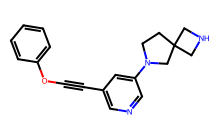
\includegraphics[width=0.9cm]{figures/gate1_structures/rank_162.png} & plain & reinvent\_pubchem & 7.61 & 5.12 & 2.27 \\
    163 & 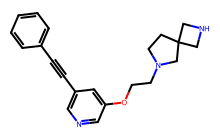
\includegraphics[width=0.9cm]{figures/gate1_structures/rank_163.png} & plain & reinvent\_pubchem & 8.05 & 5.09 & 2.16 \\
    164 & 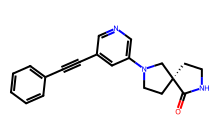
\includegraphics[width=0.9cm]{figures/gate1_structures/rank_164.png} & plain & reinvent\_pubchem & 8.17 & 5.09 & 2.20 \\
    165 & 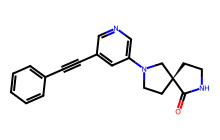
\includegraphics[width=0.9cm]{figures/gate1_structures/rank_165.png} & plain & reinvent\_pubchem & 8.17 & 5.09 & 2.20 \\
    166 & 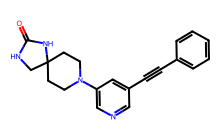
\includegraphics[width=0.9cm]{figures/gate1_structures/rank_166.png} & plain & reinvent\_pubchem & 8.17 & 5.09 & 2.13 \\
    167 & 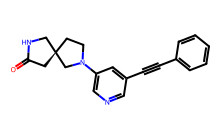
\includegraphics[width=0.9cm]{figures/gate1_structures/rank_167.png} & plain & reinvent\_pubchem & 8.17 & 5.09 & 2.20 \\
    168 & 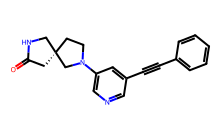
\includegraphics[width=0.9cm]{figures/gate1_structures/rank_168.png} & plain & reinvent\_pubchem & 8.17 & 5.09 & 2.20 \\
    169 & 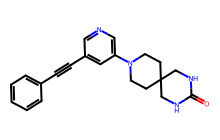
\includegraphics[width=0.9cm]{figures/gate1_structures/rank_169.png} & plain & reinvent\_pubchem & 8.17 & 5.09 & 2.38 \\
    170 & 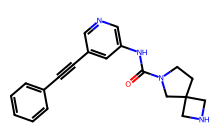
\includegraphics[width=0.9cm]{figures/gate1_structures/rank_170.png} & plain & reinvent\_pubchem & 8.17 & 5.09 & 2.31 \\
    \bottomrule
  \end{tabular}
\end{frame}

% ============================================================
\begin{frame}{Source Mode (200 compounds): Structures sorted by IC$_{50}$ (171--180)}
  \centering
  \tiny
  \begin{tabular}{r c l l c c c}
    \toprule
    \textbf{Rank} & \textbf{Structure} & \textbf{Source mode} & \textbf{Family} & \textbf{IC$_{50}$ ($\mu$M)} & \textbf{pIC$_{50}$} & \textbf{cLogP} \\
    \midrule
    171 & 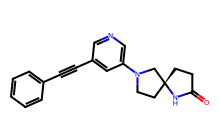
\includegraphics[width=0.9cm]{figures/gate1_structures/rank_171.png} & plain & reinvent\_pubchem & 8.17 & 5.09 & 2.34 \\
    172 & 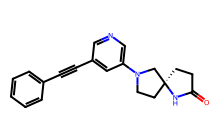
\includegraphics[width=0.9cm]{figures/gate1_structures/rank_172.png} & plain & reinvent\_pubchem & 8.17 & 5.09 & 2.34 \\
    173 & 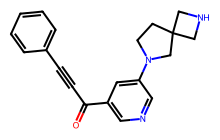
\includegraphics[width=0.9cm]{figures/gate1_structures/rank_173.png} & plain & reinvent\_pubchem & 8.17 & 5.09 & 2.12 \\
    174 & 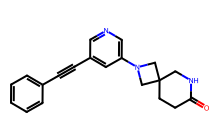
\includegraphics[width=0.9cm]{figures/gate1_structures/rank_174.png} & plain & reinvent\_pubchem & 8.17 & 5.09 & 2.20 \\
    175 & 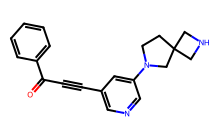
\includegraphics[width=0.9cm]{figures/gate1_structures/rank_175.png} & plain & reinvent\_pubchem & 8.17 & 5.09 & 2.12 \\
    176 & 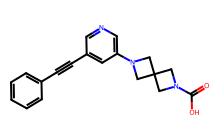
\includegraphics[width=0.9cm]{figures/gate1_structures/rank_176.png} & plain & reinvent\_pubchem & 8.36 & 5.08 & 2.28 \\
    177 & 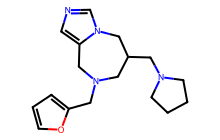
\includegraphics[width=0.9cm]{figures/gate1_structures/rank_177.png} & reinforcement\_learning & reinvent & 8.97 & 5.05 & 2.20 \\
    178 & 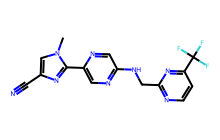
\includegraphics[width=0.9cm]{figures/gate1_structures/rank_178.png} & curriculum\_learning & reinvent & 9.12 & 5.04 & 2.17 \\
    179 & 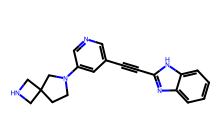
\includegraphics[width=0.9cm]{figures/gate1_structures/rank_179.png} & plain & reinvent\_pubchem & 9.36 & 5.03 & 2.16 \\
    180 & 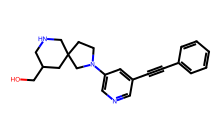
\includegraphics[width=0.9cm]{figures/gate1_structures/rank_180.png} & plain & reinvent\_pubchem & 9.40 & 5.03 & 2.28 \\
    \bottomrule
  \end{tabular}
\end{frame}

% ============================================================
\begin{frame}{Source Mode (200 compounds): Structures sorted by IC$_{50}$ (181--190)}
  \centering
  \tiny
  \begin{tabular}{r c l l c c c}
    \toprule
    \textbf{Rank} & \textbf{Structure} & \textbf{Source mode} & \textbf{Family} & \textbf{IC$_{50}$ ($\mu$M)} & \textbf{pIC$_{50}$} & \textbf{cLogP} \\
    \midrule
    181 & 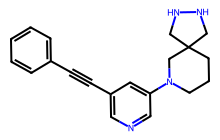
\includegraphics[width=0.9cm]{figures/gate1_structures/rank_181.png} & plain & reinvent\_pubchem & 9.80 & 5.01 & 2.18 \\
    182 & 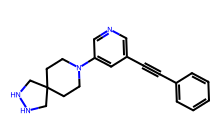
\includegraphics[width=0.9cm]{figures/gate1_structures/rank_182.png} & plain & reinvent\_pubchem & 9.80 & 5.01 & 2.18 \\
    183 & 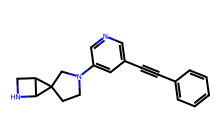
\includegraphics[width=0.9cm]{figures/gate1_structures/rank_183.png} & plain & reinvent\_pubchem & 9.81 & 5.01 & 2.28 \\
    184 & 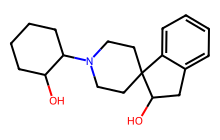
\includegraphics[width=0.9cm]{figures/gate1_structures/rank_184.png} & curriculum\_learning & reinvent & 9.81 & 5.01 & 2.24 \\
    185 & 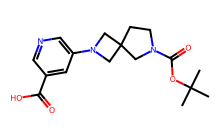
\includegraphics[width=0.9cm]{figures/gate1_structures/rank_185.png} & plain & reinvent\_pubchem & 10.14 & 4.99 & 2.23 \\
    186 & 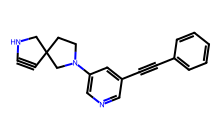
\includegraphics[width=0.9cm]{figures/gate1_structures/rank_186.png} & plain & reinvent\_pubchem & 10.19 & 4.99 & 2.24 \\
    187 & 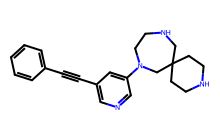
\includegraphics[width=0.9cm]{figures/gate1_structures/rank_187.png} & plain & reinvent\_pubchem & 10.35 & 4.98 & 2.26 \\
    188 & 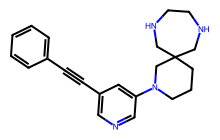
\includegraphics[width=0.9cm]{figures/gate1_structures/rank_188.png} & plain & reinvent\_pubchem & 10.35 & 4.98 & 2.26 \\
    189 & 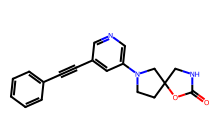
\includegraphics[width=0.9cm]{figures/gate1_structures/rank_189.png} & plain & reinvent\_pubchem & 10.48 & 4.98 & 2.17 \\
    190 & 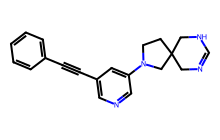
\includegraphics[width=0.9cm]{figures/gate1_structures/rank_190.png} & plain & reinvent\_pubchem & 10.48 & 4.98 & 2.31 \\
    \bottomrule
  \end{tabular}
\end{frame}

% ============================================================
\begin{frame}{Source Mode (200 compounds): Structures sorted by IC$_{50}$ (191--200)}
  \centering
  \tiny
  \begin{tabular}{r c l l c c c}
    \toprule
    \textbf{Rank} & \textbf{Structure} & \textbf{Source mode} & \textbf{Family} & \textbf{IC$_{50}$ ($\mu$M)} & \textbf{pIC$_{50}$} & \textbf{cLogP} \\
    \midrule
    191 & 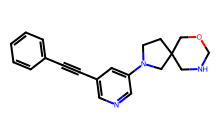
\includegraphics[width=0.9cm]{figures/gate1_structures/rank_191.png} & plain & reinvent\_pubchem & 10.48 & 4.98 & 2.26 \\
    192 & 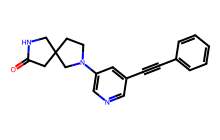
\includegraphics[width=0.9cm]{figures/gate1_structures/rank_192.png} & plain & reinvent\_pubchem & 10.48 & 4.98 & 2.20 \\
    193 & 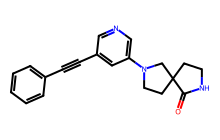
\includegraphics[width=0.9cm]{figures/gate1_structures/rank_193.png} & plain & reinvent\_pubchem & 10.48 & 4.98 & 2.20 \\
    194 & 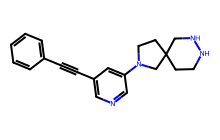
\includegraphics[width=0.9cm]{figures/gate1_structures/rank_194.png} & plain & reinvent\_pubchem & 10.48 & 4.98 & 2.18 \\
    195 & 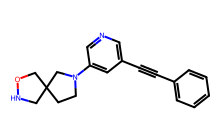
\includegraphics[width=0.9cm]{figures/gate1_structures/rank_195.png} & plain & reinvent\_pubchem & 10.48 & 4.98 & 2.21 \\
    196 & 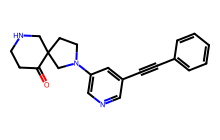
\includegraphics[width=0.9cm]{figures/gate1_structures/rank_196.png} & plain & reinvent\_pubchem & 10.48 & 4.98 & 2.24 \\
    197 & 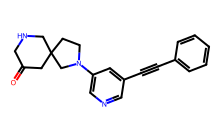
\includegraphics[width=0.9cm]{figures/gate1_structures/rank_197.png} & plain & reinvent\_pubchem & 10.48 & 4.98 & 2.24 \\
    198 & 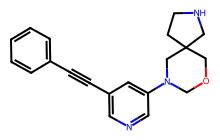
\includegraphics[width=0.9cm]{figures/gate1_structures/rank_198.png} & plain & reinvent\_pubchem & 10.48 & 4.98 & 2.26 \\
    199 & 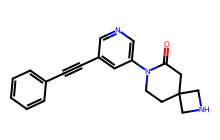
\includegraphics[width=0.9cm]{figures/gate1_structures/rank_199.png} & plain & reinvent\_pubchem & 10.72 & 4.97 & 2.20 \\
    200 & 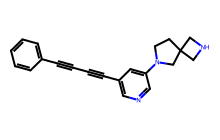
\includegraphics[width=0.9cm]{figures/gate1_structures/rank_200.png} & plain & reinvent\_pubchem & 11.55 & 4.94 & 2.28 \\
    \bottomrule
  \end{tabular}
\end{frame}
